\documentclass[dvipdfmx,autodetect-engine]{jsarticle}
\usepackage{tikz}
\usepackage{url}
\usepackage{hyperref}
\usepackage{amsmath,amssymb}
\usepackage{comment}

% see https://doratex.hatenablog.jp/entry/20180503/1525338512

\title{フィナンシャルエンジニアリング特論第2\\中間レポート}
\author{内海佑麻\footnote{学籍番号: 82018398 所属: 理工学研究科 環境開放科学専攻 情報工学専修 連絡先: uchiumi@ailab.ics.keio.ac.jp} 
    \and 澤屋敷友一\footnote{学籍番号: 82019220 所属: 理工学研究科 環境開放科学専攻 オープンシステムマネジメント専修 連絡先: yashiki@keio.jp }}
\date{November 27, 2020}

\begin{document}

\maketitle

\begin{abstract}
代表的なポートフォリオ選択モデルとしてMarkowitzの平均分散モデルとシャープレシオ最大化モデルを構築して資産運用を行う金融商品(ポートフォリオ)を組成した.東京証券取引所の内国株式を運用対象とし,ヒストリカルデータに対してバックテストを行い,運用結果に対するモデル間比較やそれぞれのモデルがもつ性質について考察を行った.
\end{abstract}

\tableofcontents

\newpage

\section{モデルの構築方法}

\subsection{ポートフォリオ選択モデル}

\subsubsection{Markowitzの平均分散モデル}

Markowitzの平均分散モデルでは,「ポートフォリオの期待収益率(Expected return)が一定値以上となる」という制約条件の下で,「ポートフォリオの分散を最小化する」最適化問題を考える.一般に,$n$コの資産で構成されるポートフォリオの場合,ポートフォリオの分散は$n$コの資産間の共分散行列の二次形式となるので,この最適化問題は二次計画問題(Quadratic Programming, QP)のクラスとなり,次のように定式化される.
\begin{align}
    \underset{\bf x \in \mathcal{X}}{\rm minimize} ~~~ 
    &\sigma_p \left( = {\bf x}^{\mathrm{T}} \Sigma {\bf x} \right) \\
    {\rm subject~to} ~~~ &\bar{r}_p = \bar{\bf r}^{\mathrm{T}} {\bf x} = \sum_{i=1}^{n} \bar{r}_i x_i \geq r_e \\
    &{\| {\bf x} \|}_{1} = \sum_{i=1}^{n} x_i = 1 \\
    &x_i \geq 0 ~~ (i = 1, \cdots, n)
\end{align}

\begin{itemize}
    \item $\Sigma \in \mathbb{R}^{n \times n}$ - $n$コの資産の共分散行列
    \item ${\bf x} \in \mathbb{R}^{n}$ - $n$コの資産の投資比率ベクトル
    \item $\bar{\bf r} \in \mathbb{R}^{n}$ - $n$コの資産の期待収益率ベクトル
    \item $x_i \in \mathbb{R}$ - 資産$i$の投資比率
    \item $\bar{r}_i \in \mathbb{R}$ - 資産$i$の期待収益率
    \item $r_e \in \mathbb{R}$ - 投資家の要求期待収益率
    \item $\bar{r}_p \in \mathbb{R}$ - ポートフォリオの期待収益率
    \item $\sigma_p \in \mathbb{R}$ - ポートフォリオの標準偏差
\end{itemize}
1つ目の制約式は,ポートフォリオの期待収益率が一定値($=r_e$)以上となることを要請している.2つ目,3つ目の制約式はポートフォリオの定義からくる自明なものである.資産の空売りを許す場合,3つ目の制約式を除くこともある.

\subsubsection{Sharpe-ratio最大化モデル}

シャープレシオ(Sharpe ratio, SR)は,最もよく使われるポートフォリオに対するリスク調整済みパフォーマンス尺度である.任意のポートフォリオ$p$のシャープレシオ${\theta}_p$は,無リスク資産の収益率$r_f$とポートフォリオの期待収益率$\bar{r}_p$,ポートフォリオの標準偏差$\sigma_p$を用いて
\begin{align}
    {\theta}_p := \frac{\bar{r}_p - r_f}{\sigma_p}
\end{align}
と定義される.シャープレシオ最大化問題は,
目的関数に$n$コの資産間の共分散行列が含まれるため,二次計画問題(Quadratic Programming, QP)のクラスとなり,次のように定式化される.

\begin{align}
    \underset{\bf x \in \mathcal{X}}{\rm maximize} ~~~ 
    &\frac{\bar{r}_p - r_f}{\sigma_p}
    \left( 
    = \frac{\bar{\bf r}^{\mathrm{T}} {\bf x} - r_f}{\sqrt{{\bf x}^{\mathrm{T}} \Sigma {\bf x}}}
    \right) \\
    {\rm subject~to} ~~~ 
    &{\| {\bf x} \|}_{1} = \sum_{i=1}^{n} x_i = 1 \\
    &x_i \geq 0 ~~ (i = 1, \cdots, n)
\end{align}

\begin{itemize}
    \item $r_f \in \mathbb{R}$ - 無リスク資産の収益率
\end{itemize}

上式の目的関数を二次形式で表すため,ポートフォリオの期待リスクプレミアム$\lambda$と各資産の比重ベクトル${\bf w} = {\bf x} / \lambda$を導入して変形すると,次のようにSharpe-ratio最大化問題のコンパクト分解表現を得る.

\begin{align}
    \underset{\bf w \in \mathcal{W}}{\rm minimize} ~~~ 
    & {\bf w}^{\mathrm{T}} \Sigma {\bf w} \\
    {\rm subject~to} ~~~ 
    &{\| \hat{\bf r}^{\mathrm{T}} {\bf w} \|}_{1} = \sum_{i=1}^{n} (\bar{r}_i - r_f) w_i = 1 \\
    &w_i \geq 0 ~~ (i = 1, \cdots, n)
\end{align}

\begin{itemize}
    \item $x_i \in \mathbb{R}$ - 資産$i$の投資比率
    \item $w_i \in \mathbb{R}$ - 資産$i$の投資比率と期待リスクプレミアムの比率 ($w_i = x_i / \lambda $)
    \item $\lambda \in \mathbb{R}$ - ポートフォリオの期待リスクプレミアム ($\lambda = \sum_{i=1}^{n} \hat{r}_i x_i = \sum_{i=1}^{n} (\bar{r}_i - r_f) x_i$)
    \item $\hat{r}_i \in \mathbb{R}$ - 資産$i$の期待リスクプレミアム ($\hat{r}_i = \bar{r}_i - r_f$)
\end{itemize}

ここで,定義式$x_i = \lambda w_i$と予算制約式$\sum_{i=1}^{n} x_i = 1$に注意すると,$\lambda = 1/(\sum_{i=1}^{n} w_i)$となるから,元問題の実行可能解$\bf x$とコンパクト分解表現の実行可能解$\bf w$の間に以下のような1対1対応が成り立つ.

\begin{align}
    {\bf x} = \lambda {\bf w} =  \frac{\bf w}{\sum_{i=1}^{n} w_i} = \frac{\bf w}{{\|{\bf w}\|}_1}
\end{align}


\subsection{ソフトウェアとデータ}

Pythonを用いてポートフォリオ選択モデルの実装とヒストリカルデータに対するバックテストを行った.今回作成したPythonスクリプトではすでに公開されているパッケージを使っていない.主な理由は,資産運用やシステムトレード向けのPythonパッケージはいくつかあるが,米国の株式市場を対象としたものが多く,日本の株式市場に対応しているものは少ないためである.\footnote{"The Top 22 Python Trading Tools for 2020", \url{https://analyzingalpha.com/python-trading-tools}}また,作成したスクリプトや実行ファイルはGithub上にリポジトリ(\url{https://github.com/yumaloop/afe2_backtest}
)として公開した.

\subsubsection{pandas-datareaderパッケージによるデータ取得}

株式銘柄のヒストリカルデータは,pandas-datareaderを用いて取得した.pandas-datareaderは,IEX, World Bank, OECD, Yahoo! Finance,FRED,Stooqなどが公開しているWeb APIを内部で呼び出すことで、Pythonスクリプト上に取得したいデータを読み込みことができる.

\subsubsection{cvxoptパッケージによる二次計画問題の球解}

銘柄選択時に必要となる凸最適化問題の球解には,cvxopt (\url{https://cvxopt.org})を使った.cvxoptは二次計画問題(QP)を含む一般の凸最適化問題に対する高速ソルバである.cvxoptで二次計画問題を扱う場合は,解きたい最適化問題を以下の一般形式に整理して,

\begin{align}
\underset{{\bf x} \in \mathcal{X}}{\rm minimize} ~~~ 
&\frac{1}{2} {\bf x}^{\mathrm{T}} P {\bf x} + {\bf q}^{\mathrm{T}} {\bf x} \\
{\rm subject~to} ~~~ & G {\bf x} \leq {\bf h} \\
&A {\bf x} = {\bf b}
\end{align}

パラメータ$P,q,G,h,A$を計算し,\href{https://cvxopt.org/userguide/coneprog.html#quadratic-programming}{cvxopt.solvers.qp()}関数を実行することで最適解と最適値を求める.たとえば,Markowitzの平均・分散モデルの場合は,

\begin{align}
    P = 2 \cdot \Sigma, \hspace{1em}
    q = {\bf 0}_n, \hspace{1em}
    G = -1 \cdot
        \begin{pmatrix}
            \bar{r}_1 & \cdots & \bar{r}_n \\
            1 & \cdots & 0 \\
            \vdots & \ddots & \vdots \\
            0 & \cdots & 1 
        \end{pmatrix}, \hspace{1em}
    h = -1 \cdot 
        \left(
            \begin{array}{c}
              r_e \\
              0 \\
              \vdots \\
              0
            \end{array}
        \right), \hspace{1em}
    A = {\bf 1}_n^{\mathrm{T}}, \hspace{1em}
    b = 1
\end{align}

となり\footnote{cvxoptの公式ドキュメント参照.\url{https://cvxopt.org/userguide/coneprog.html\#quadratic-programming}},シャープレシオ最大化モデルの場合は次のようになる.

\begin{align}
    P = 2 \cdot \Sigma, \hspace{1em}
    q = {\bf 0}_n, \hspace{1em}
    G = -1 \cdot
        \begin{pmatrix}
            1 & \cdots & 0 \\
            \vdots & \ddots & \vdots \\
            0 & \cdots & 1 
        \end{pmatrix}, \hspace{1em}
    h = {\bf 0}_n, \hspace{1em}
    A = {\left(
            \begin{array}{c}
              \bar{r}_1 - r_f \\
              \vdots \\
              \bar{r}_n - r_f
            \end{array}
        \right)}^{\mathrm{T}}, \hspace{1em}
    b = 1
\end{align}

\subsection{バックテストの設定}

以下のような設定下で,ポートフォリオ選択モデルを過去の価格データへ適用し,バックテストを行った.

\begin{itemize}
    \item 運用期間 \hspace{0.05em} - \hspace{0.05em} 
    2011年10月31日~2020年10月31日 (過去10年間)\footnote{.TOPIXシリーズの構成銘柄は毎年10/31に更新されるため10/31を基準日とした.}
    \item 対象資産 \hspace{0.05em} - \hspace{0.05em} 
    運用開始時点(2011年10月31日)で,TOPIX 500 (Core30)に採用されている内国株式
    \item 無リスク資産の利回り \hspace{0.05em} - \hspace{0.05em} 
    0.01\% 日本国債10年物利回り\footnote{出典: Bloomberg LP, \url{https://www.bloomberg.co.jp/markets/rates-bonds/government-bonds/japan}}
    \item リバランス単位 \hspace{0.05em} - \hspace{0.05em} 
    1カ月ごとにポートフォリオを再調整する.
    \item パラメータの推定期間 \hspace{0.05em} - \hspace{0.05em} 
    リバランス時点から過去36カ月
    \item パフォーマンス評価 \hspace{0.05em} - \hspace{0.05em} 
    運用期間におけるポートフォリオのシャープレシオ(年率)
\end{itemize}

\section{バックテストとパフォーマンス評価}

\subsection{運用期間における東京証券取引所の動向}

東証TOPIXシリーズの構成銘柄に対して収益率および累積収益率の変動をみると,2007-2009の大きな下降,2012-2013の大きな上昇を除くと緩やかに増加していることがわかる.

\begin{figure}[htbp]
    \begin{minipage}{0.5\hsize}
        \begin{center}
            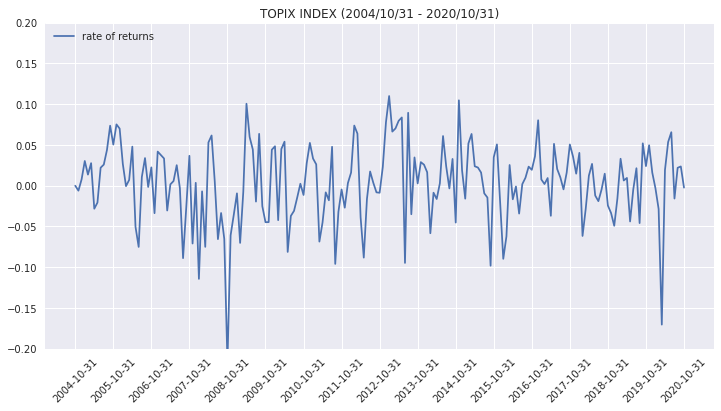
\includegraphics[width=1.0\hsize]{./figures/topixindex_chg_20041031-20201031.png}
            \caption{TOPIX Indexの収益率}
            \label{fig:one}
        \end{center}
    \end{minipage}
    \begin{minipage}{0.5\hsize}
        \begin{center}
            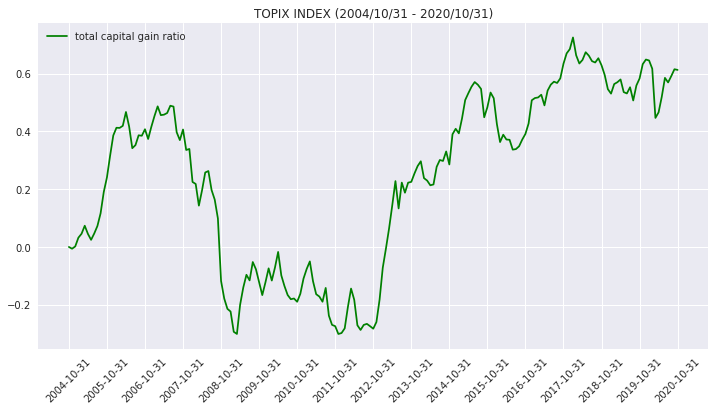
\includegraphics[width=1.0\hsize]{./figures/topixindex_cum_20041031-20201031.png}
            \caption{TOPIX Indexの累積収益率}
            \label{fig:two}
        \end{center}
    \end{minipage}
\end{figure}

\begin{figure}[htbp]
    \begin{minipage}{0.5\hsize}
        \begin{center}
            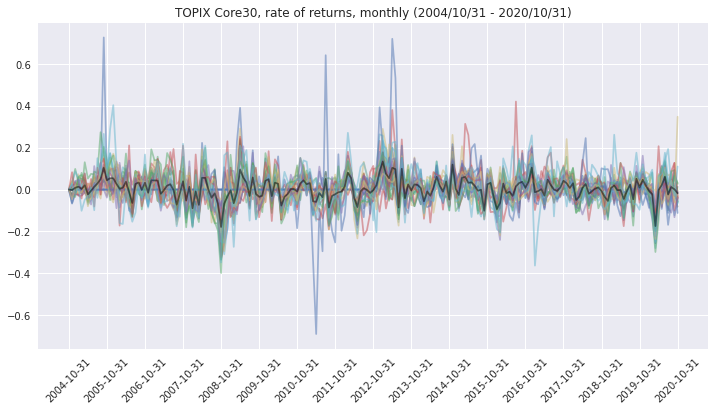
\includegraphics[width=1.0\hsize]{./figures/topixcore30_chg_20041031-20201031.png}
            \caption{TOPIX Core30構成銘柄の収益率}
            \label{fig:one}
        \end{center}
    \end{minipage}
    \begin{minipage}{0.5\hsize}
        \begin{center}
            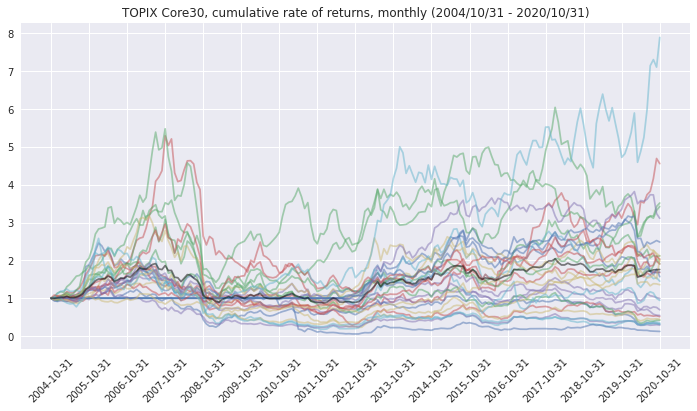
\includegraphics[width=1.0\hsize]{./figures/topixcore30_cum_20041031-20201031.png}
            \caption{TOPIX Core30構成銘柄の累積収益率}
            \label{fig:two}
        \end{center}
    \end{minipage}
\end{figure}

\begin{figure}[htbp]
    \begin{minipage}{0.5\hsize}
        \begin{center}
            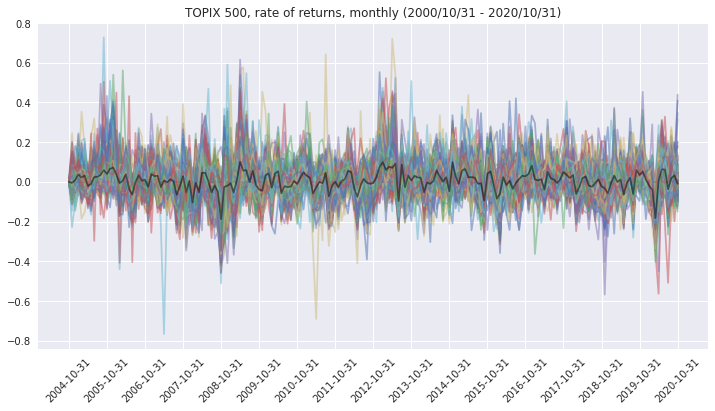
\includegraphics[width=1.0\hsize]{./figures/topix500_chg_20041031-20201031.png}
            \caption{TOPIX 500構成銘柄の収益率}
            \label{fig:one}
        \end{center}
    \end{minipage}
    \begin{minipage}{0.5\hsize}
        \begin{center}
            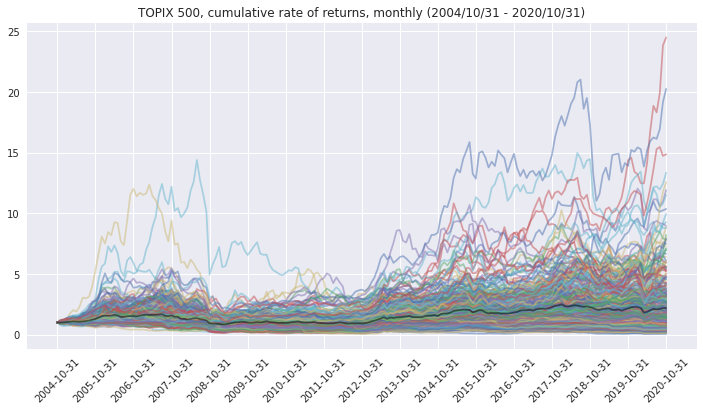
\includegraphics[width=1.0\hsize]{./figures/topix500_cum_20041031-20201031.png}
            \caption{TOPIX 500構成銘柄の累積収益率}
            \label{fig:two}
        \end{center}
    \end{minipage}
\end{figure}

実際,収益率のヒストグラムをみると,平均が正となる単峰性の形状を示しており,「収益率は正規分布に従う確率変数である」と仮定することが妥当であると判断できる.すなわち,平均・分散をリターン・リスクの計算に用いることが正当化される.

\begin{figure}[htbp]
    \begin{center}
        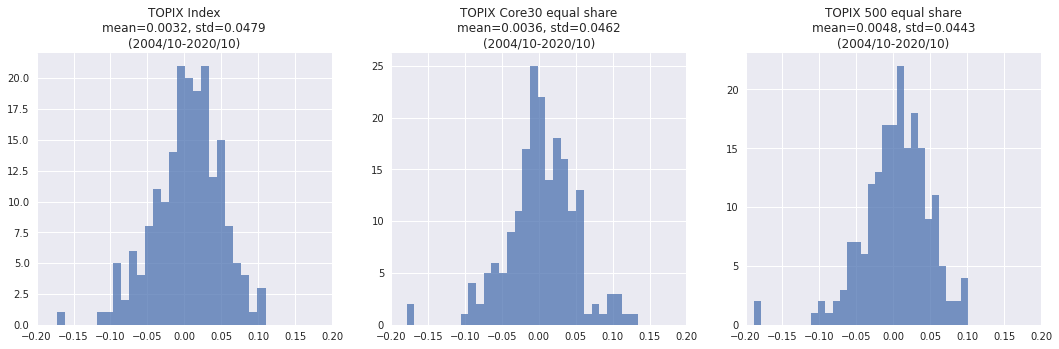
\includegraphics[width=0.95\hsize]{./figures/topix_ror_dist_20041031-20201031.png}
        \caption{TOPIXシリーズの月次収益率分布
        (期間:2004/10 - 2020/10): 
        (1) TOPIX Index(東証全銘柄に対する加重平均)
        (2) TOPIX Core30構成銘柄に対する等配分ポートフォリオ
        (3) TOPIX 500構成銘柄に対する等配分ポートフォリオ}
        \label{fig:two}
    \end{center}
\end{figure}

\subsection{ポートフォリオ選択モデルのパフォーマンス比較}

\begin{table}[htb]
    \caption{バックテストの結果: 運用期間:2011/10 - 2020/10 (年率)}
    \label{table:backtest_result}
    \centering
    \begin{tabular}{lccc}
        \hline
        ポートフォリオ選択モデル & シャープレシオ & リターン & リスク \\
        (対象銘柄, パラメータ推定期間) & $\theta_p$ & $\bar{r}_p$ & $\sigma_p$ \\
        \hline \hline
        平均分散モデル(TOPIX C30, 12カ月) & 0.5691 & 0.0920 & 0.1615 \\
        平均分散モデル(TOPIX C30, 36カ月) & 0.6509 & 0.0882 & 0.1354 \\
        平均分散モデル(TOPIX C30, 60カ月) & 0.6059 & 0.0848 & 0.1398 \\
        シャープレシオ最大化モデル(TOPIX C30, 12カ月) & 0.6181 & 0.1121 & 0.1812 \\
        シャープレシオ最大化モデル(TOPIX C30, 36カ月) & 0.7335 & 0.1245 & 0.1697 \\
        シャープレシオ最大化モデル(TOPIX C30, 60カ月) & 0.6604 & 0.1201 & 0.1817 \\
        東証TOPIX C30 等配分ポートフォリオ & 0.2777 & 0.4911 & 1.7684 \\ 
        東証TOPIX 500 等配分ポートフォリオ & 0.4966 & 0.0852 & 0.1716 \\ 
        東証株価指数, TOPIX INDEX & 0.5443 & 0.0887 & 0.1629 \\
        日経平均株価, Nikkei 225 & 0.6685 & 0.1085 & 0.1623 \\
        \hline
    \end{tabular}
\end{table}

平均分散モデルとシャープレシオ最大化モデルに対するバックテストの結果を表\ref{table:backtest_result}に示す\footnote{平均分散モデルに与える要求期待収益率はパラメータ推定期間におけるTOPIX Indexの平均収益率とした.}\footnote{東証株価指数: 東証1部上場の全銘柄を対象として浮動株数に基づく時価総額比の加重平均.}

東京証券取引所の内国株は変動が小さく,分散最小化が適用される平均分散モデルの収益率は低い.運用期間における収益率の系列をみると,平均分散モデルはマーケット全体のトレンドとの相関が高く\footnote{パラメータ推定期間(12カ月,36カ月,60カ月)によらず,
平均分散モデルの収益率推移とTOPIX INDEXとの相関係数は,シャープレシオ最大化モデルとTOPIX INDEXとの相関係数よりも大きい.},市場全体が下落トレンドの時期(2015年-2016年)に平均分散モデルによるポートフォリオの収益率も下落していることがわかる.また,投資対象資産の特性を推定する期間については,平均分散モデル,シャープレシオ最大化モデルともに過去36カ月に基づく推定のパフォーマンスが優れていた.

% \begin{figure}[hb]
% \begin{center}
% 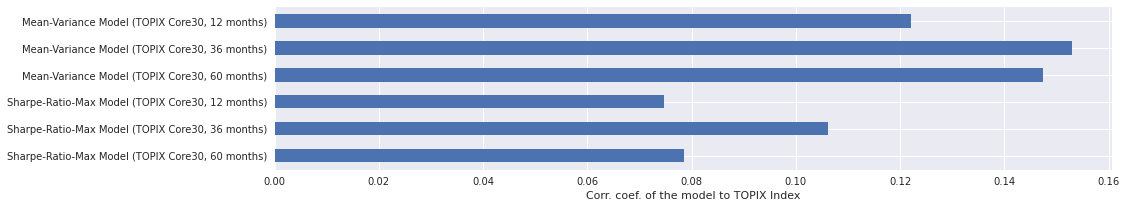
\includegraphics[width=0.75\hsize]{./figures/vs_tpx_corrcoef.png}
% \caption{ポートフォリオ運用期間における各投資戦略の収益率とTOPIX Indexとの相関係数}
% \label{fig:corrcoef_tpx}
% \end{center}
% \end{figure}


\begin{figure}[htbp]
\begin{minipage}{0.5\hsize}
\begin{center}
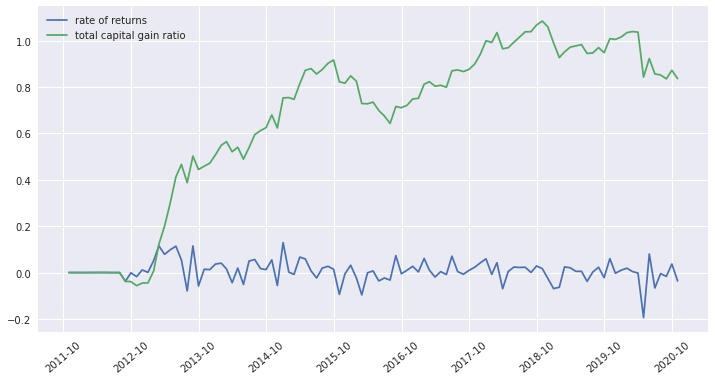
\includegraphics[width=1.0\hsize]{./figures/mmvp_tpx30_w=12_plot.png}
\end{center}
\caption{\small 平均分散モデル [$\theta_p=0.5691$]\\(TOPIX Core30構成銘柄, 推定期間:12カ月)}
\label{fig:11}
\end{minipage}
\begin{minipage}{0.5\hsize}
\begin{center}
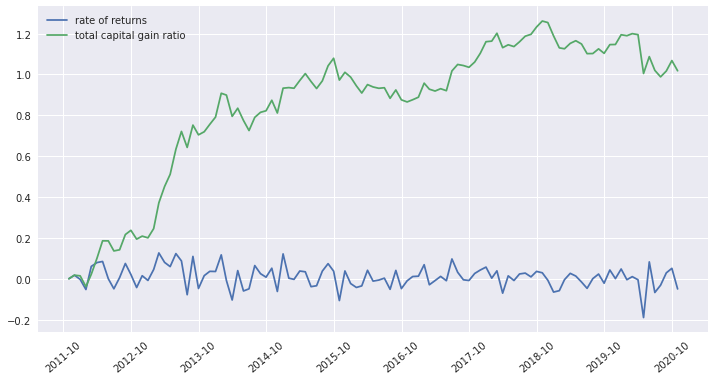
\includegraphics[width=1.0\hsize]{./figures/srmp_tpx30_w=12_plot.png}
\end{center}
\caption{\small シャープレシオ最大化モデル [$\theta_p=0.6181$]\\(TOPIX Core30構成銘柄, 推定期間:12カ月)}
\label{fig:12}
\end{minipage}
%%%%%%%%%%%%%%%%%%%%%%%%%%%%%%%%%%%%%%%%%%%%%%%%%%%%%%
\begin{minipage}{0.5\hsize}
\begin{center}
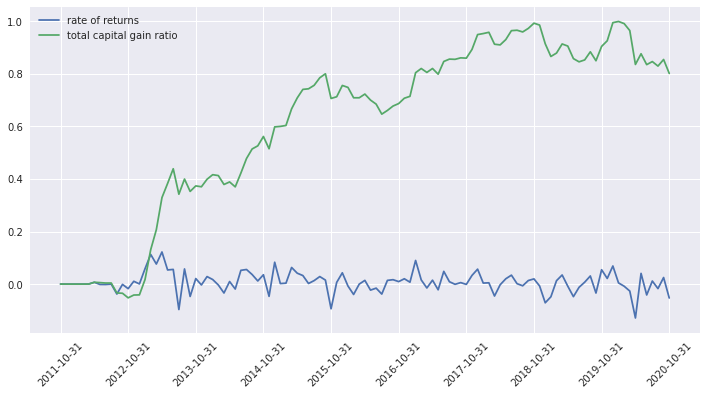
\includegraphics[width=1.0\hsize]{./figures/mmvp_tpx30_w=36_plot.png}
\end{center}
\caption{\small 平均分散モデル [$\theta_p=0.6509$]\\(TOPIX Core30構成銘柄, 推定期間:36カ月)}
\label{fig:21}
\end{minipage}
\begin{minipage}{0.5\hsize}
\begin{center}
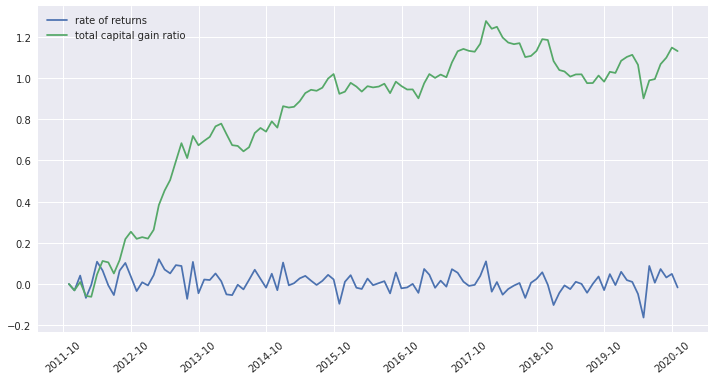
\includegraphics[width=1.0\hsize]{./figures/srmp_tpx30_w=36_plot.png}
\end{center}
\caption{\small シャープレシオ最大化モデル [$\theta_p=0.7335$]\\(TOPIX Core30構成銘柄, 推定期間:36カ月)}
\label{fig:22}
\end{minipage}
%%%%%%%%%%%%%%%%%%%%%%%%%%%%%%%%%%%%%%%%%%%%%%%%%%%%%%
\begin{minipage}{0.5\hsize}
\begin{center}
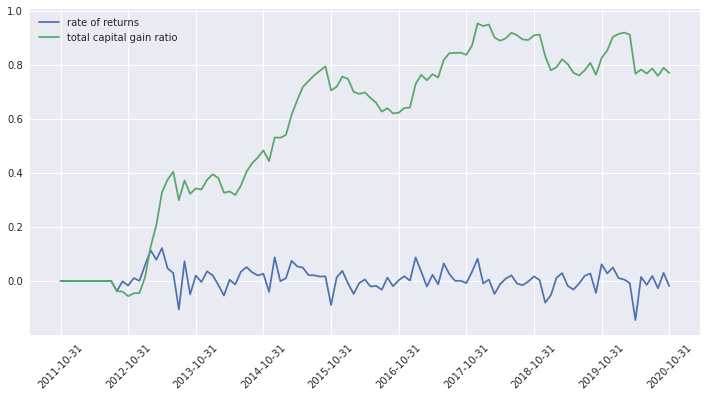
\includegraphics[width=1.0\hsize]{./figures/mmvp_tpx30_w=60_plot.png}
\end{center}
\caption{\small 平均分散モデル [$\theta_p=0.6059$]\\(TOPIX Core30構成銘柄, 推定期間:60カ月)}
\label{fig:31}
\end{minipage}
\begin{minipage}{0.5\hsize}
\begin{center}
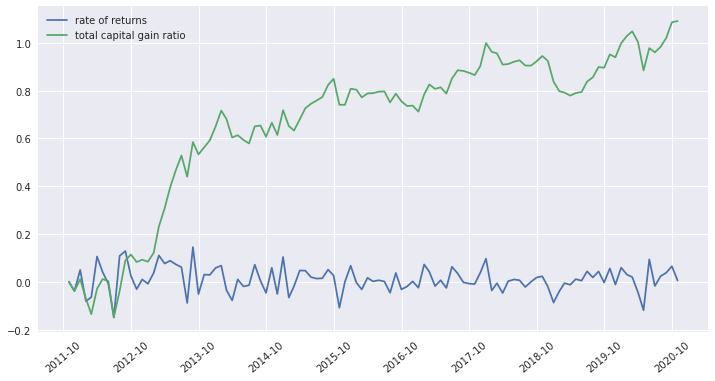
\includegraphics[width=1.0\hsize]{./figures/srmp_tpx30_w=60_plot.png}
\end{center}
\caption{\small シャープレシオ最大化モデル [$\theta_p=0.6604$]\\(TOPIX Core30構成銘柄, 推定期間:60カ月)}
\label{fig:32}
\end{minipage}
\end{figure}

\newpage

月次収益率の分布をみると,平均分散モデルは分布形状が急尖的である一方,シャープレシオ最大モデルは分布形状が緩尖的である.すなわち3次モーメント(歪度, skewness)や4次モーメント(尖度, kurtosis)をリスク尺度の特性値として用いることが有用であることが推察される.

\begin{figure}[htbp]
\begin{minipage}{0.5\hsize}
\begin{center}
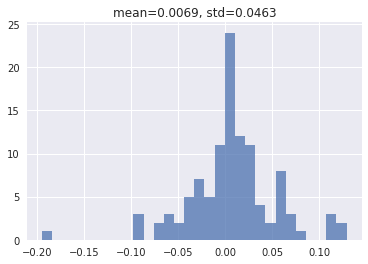
\includegraphics[width=1.0\hsize]{./figures/mmvp_tpx30_w=12_hist.png}
\end{center}
\caption{\small 月次収益率分布, 平均分散モデル\\(TOPIX Core30構成銘柄, 推定期間:12カ月)}
\label{fig:11}
\end{minipage}
\begin{minipage}{0.5\hsize}
\begin{center}
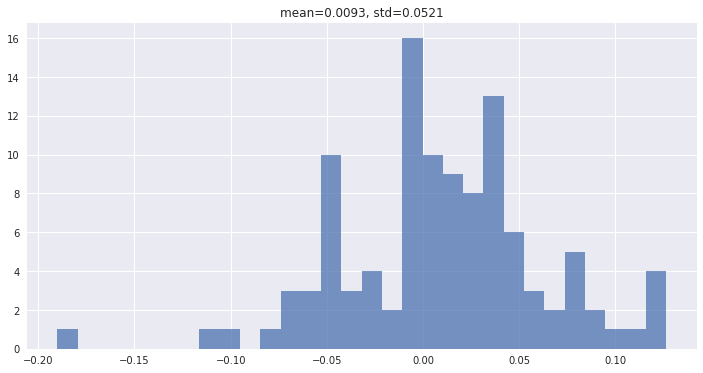
\includegraphics[width=1.0\hsize]{./figures/srmp_tpx30_w=12_hist.png}
\end{center}
\caption{\small 月次収益率分布, シャープレシオ最大化モデル(TOPIX Core30構成銘柄, 推定期間:12カ月)}
\label{fig:12}
\end{minipage}
%%%%%%%%%%%%%%%%%%%%%%%%%%%%%%%%%%%%%%%%%%%%%%%%%%%%%%
\begin{minipage}{0.5\hsize}
\begin{center}
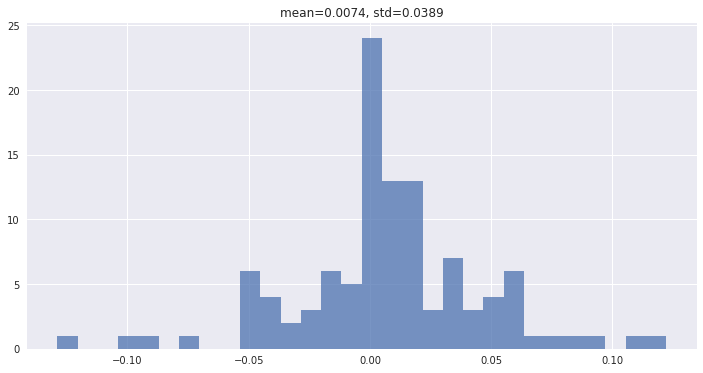
\includegraphics[width=1.0\hsize]{./figures/mmvp_tpx30_w=36_hist.png}
\end{center}
\caption{\small 月次収益率分布, 平均分散モデル\\(TOPIX Core30構成銘柄, 推定期間:36カ月)}
\label{fig:21}
\end{minipage}
\begin{minipage}{0.5\hsize}
\begin{center}
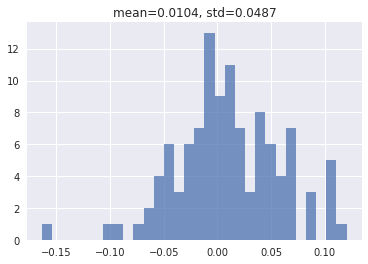
\includegraphics[width=1.0\hsize]{./figures/srmp_tpx30_w=36_hist.png}
\end{center}
\caption{\small 月次収益率分布, シャープレシオ最大化モデル(TOPIX Core30構成銘柄, 推定期間:36カ月)}
\label{fig:22}
\end{minipage}
%%%%%%%%%%%%%%%%%%%%%%%%%%%%%%%%%%%%%%%%%%%%%%%%%%%%%%
\begin{minipage}{0.5\hsize}
\begin{center}
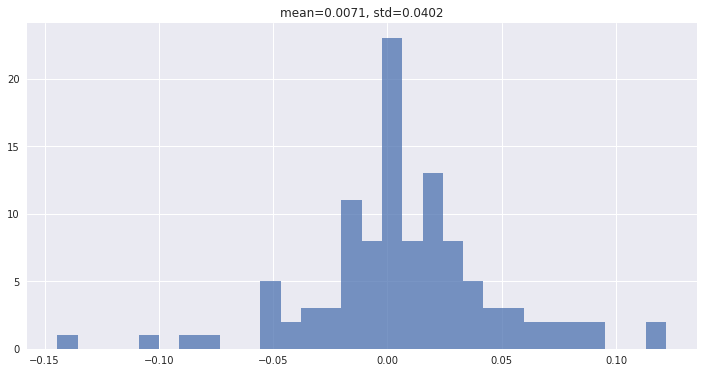
\includegraphics[width=1.0\hsize]{./figures/mmvp_tpx30_w=60_hist.png}
\end{center}
\caption{\small 月次収益率分布, 平均分散モデル\\(TOPIX Core30構成銘柄, 推定期間:60カ月)}
\label{fig:31}
\end{minipage}
\begin{minipage}{0.5\hsize}
\begin{center}
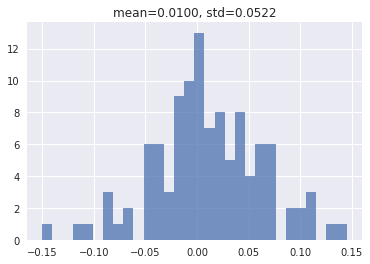
\includegraphics[width=1.0\hsize]{./figures/srmp_tpx30_w=60_hist.png}
\end{center}
\caption{\small 月次収益率分布, シャープレシオ最大化モデル(TOPIX Core30構成銘柄, 推定期間:60カ月)}
\label{fig:32}
\end{minipage}
\end{figure}

\newpage

今回組成した6つのポートフォリオを比較する.2013年と2017年はTOPIX Core30に上昇トレンドがあり,すべてのポートフォリオでパフォーマンスが良い.2014年・2015年は大きな収益率の変動こそないが,安定したパフォーマンスを維持している.
市場全体が高ボラティリティに晒された2012年・2020年のパフォーマンスで平均分散モデルとシャープレシオ最大化モデルに差がでている.

\begin{figure}[htbp]
\begin{minipage}{1.0\hsize}
    \begin{center}
        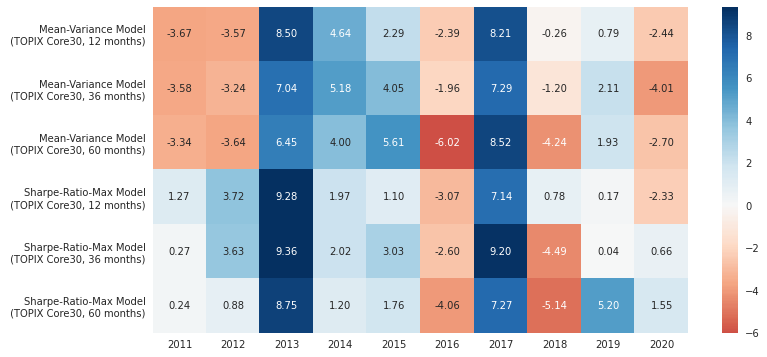
\includegraphics[width=0.75\hsize]{./figures/portfolio_sharperatio_hm.png}
        \caption{\small ポートフォリオの比較: 年次シャープレシオ}
        \label{fig:31}
    \end{center}
\end{minipage}
%%%%%%%%%%%%%%%%%%%%%%%%%%%%%%%%%%%%%%%%%%%%%%%%%%%%%%
\begin{minipage}{1.0\hsize}
    \begin{center}
        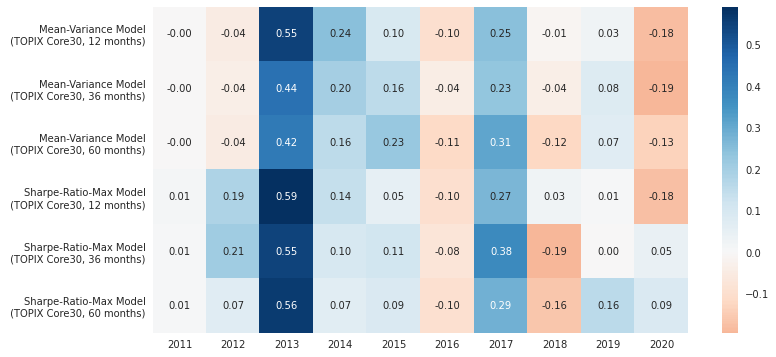
\includegraphics[width=0.75\hsize]{./figures/portfolio_returns_hm.png}
        \caption{\small ポートフォリオの比較: 年次リターン(収益率の平均)}
        \label{fig:31}
    \end{center}
\end{minipage}
%%%%%%%%%%%%%%%%%%%%%%%%%%%%%%%%%%%%%%%%%%%%%%%%%%%%%%
\begin{minipage}{1.0\hsize}
    \begin{center}
        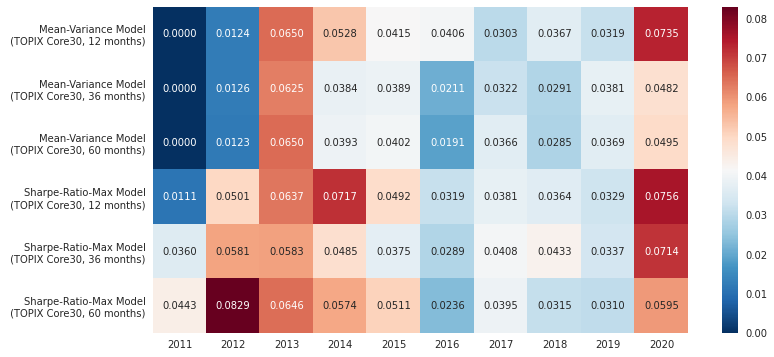
\includegraphics[width=0.75\hsize]{./figures/portfolio_risk_hm.png}
        \caption{\small ポートフォリオの比較: 年次リスク(収益率の標準偏差)}
        \label{fig:31}
    \end{center}
\end{minipage}
\end{figure}

\newpage

\begin{figure}[htbp]
\begin{minipage}{0.5\hsize}
\begin{center}
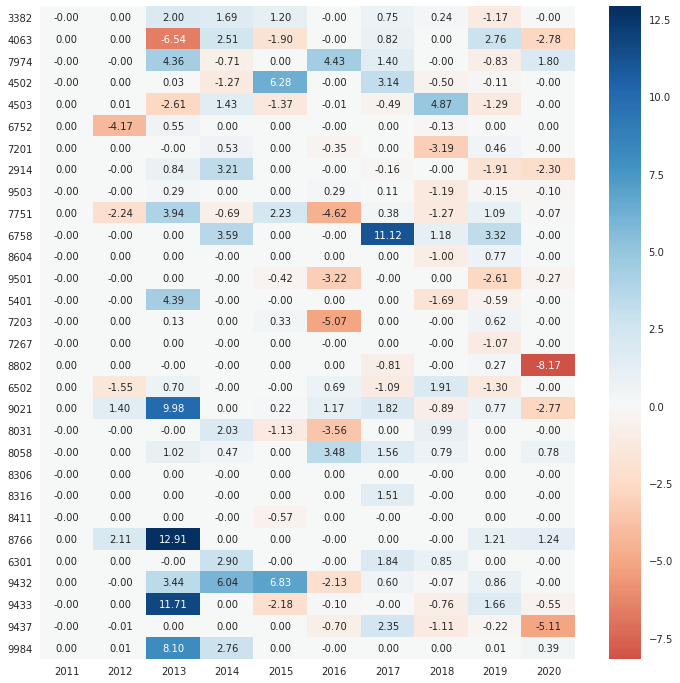
\includegraphics[width=0.8\hsize]{./figures/mmvp_tpx30_w=12_hm.png}
\end{center}
\caption{\small 各銘柄の年次収益率(\%) 平均分散モデル\\(TPX C30構成銘柄, 12カ月)}
\label{fig:11}
\end{minipage}
\begin{minipage}{0.5\hsize}
\begin{center}
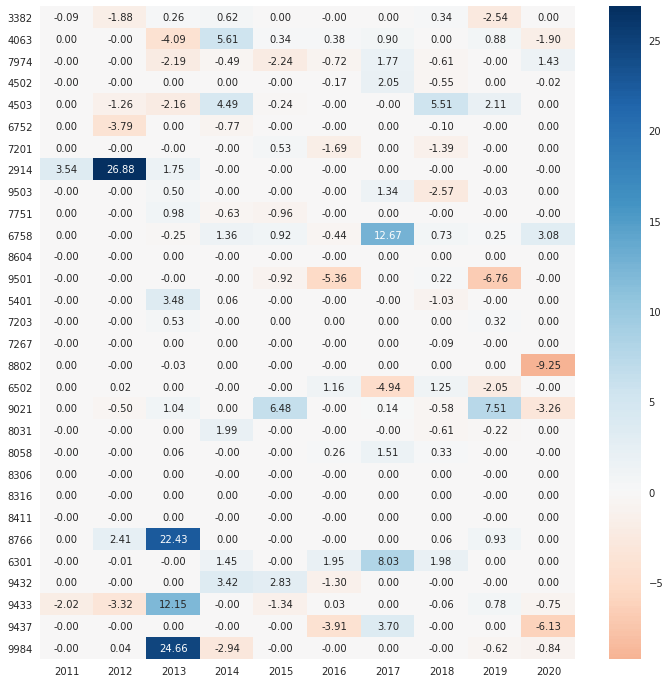
\includegraphics[width=0.8\hsize]{./figures/srmp_tpx30_w=12_hm.png}
\end{center}
\caption{\small 各銘柄の年次収益率(\%) シャープレシオ最大化モデル(TPX C30構成銘柄, 推定期間:12カ月)}
\label{fig:12}
\end{minipage}
%%%%%%%%%%%%%%%%%%%%%%%%%%%%%%%%%%%%%%%%%%%%%%%%%%%%%%
\begin{minipage}{0.5\hsize}
\begin{center}
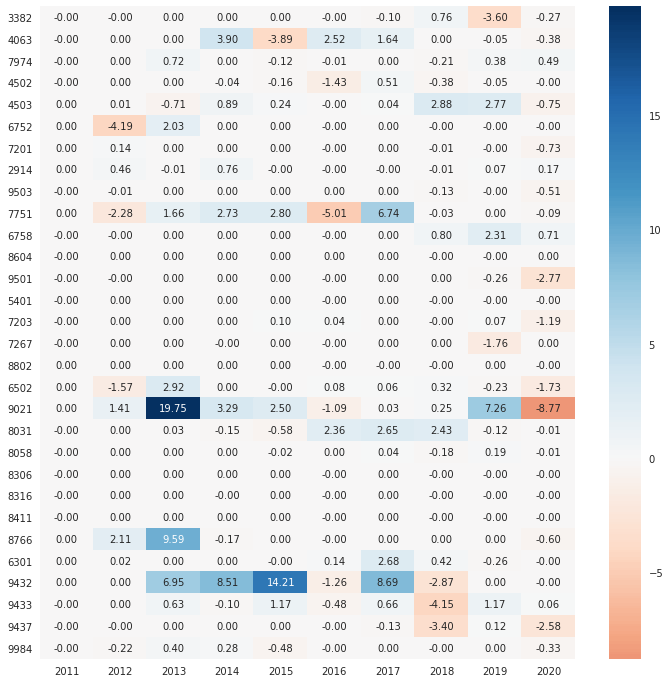
\includegraphics[width=0.8\hsize]{./figures/mmvp_tpx30_w=36_hm.png}
\end{center}
\caption{\small 各銘柄の年次収益率(\%) 平均分散モデル\\(TPX C30構成銘柄, 推定期間:36カ月)}
\label{fig:21}
\end{minipage}
\begin{minipage}{0.5\hsize}
\begin{center}
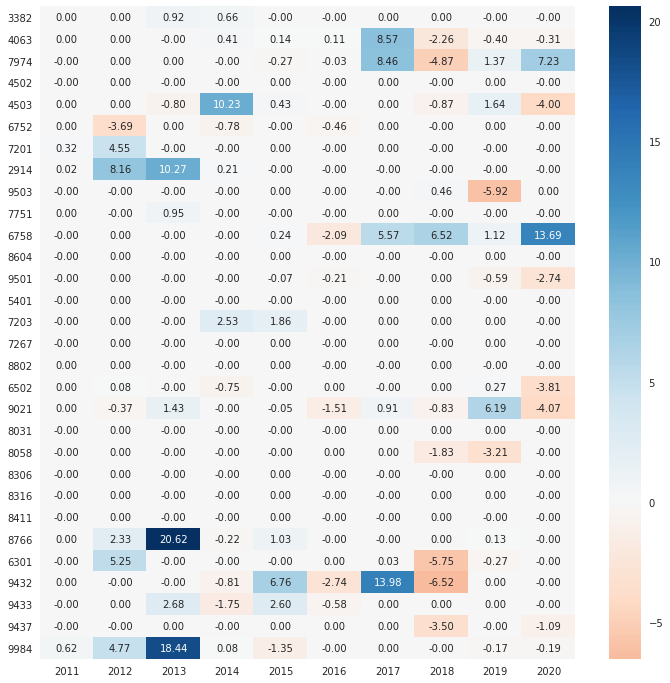
\includegraphics[width=0.8\hsize]{./figures/srmp_tpx30_w=36_hm.png}
\end{center}
\caption{\small 各銘柄の年次収益率(\%) シャープレシオ最大化モデル(TPX C30構成銘柄, 推定期間:36カ月)}
\label{fig:22}
\end{minipage}
%%%%%%%%%%%%%%%%%%%%%%%%%%%%%%%%%%%%%%%%%%%%%%%%%%%%%%
\begin{minipage}{0.5\hsize}
\begin{center}
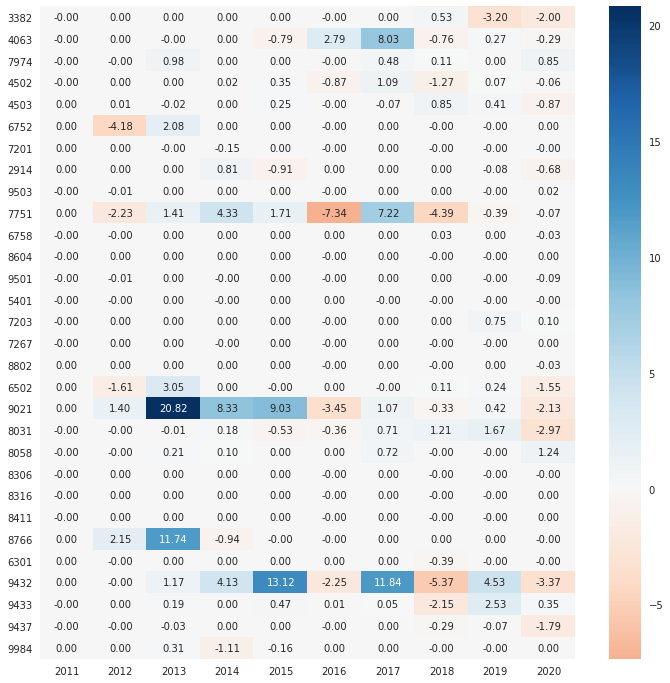
\includegraphics[width=0.8\hsize]{./figures/mmvp_tpx30_w=60_hm.png}
\end{center}
\caption{\small 各銘柄の年次収益率(\%) 平均分散モデル\\(TPX C30構成銘柄, 推定期間:60カ月)}
\label{fig:31}
\end{minipage}
\begin{minipage}{0.5\hsize}
\begin{center}
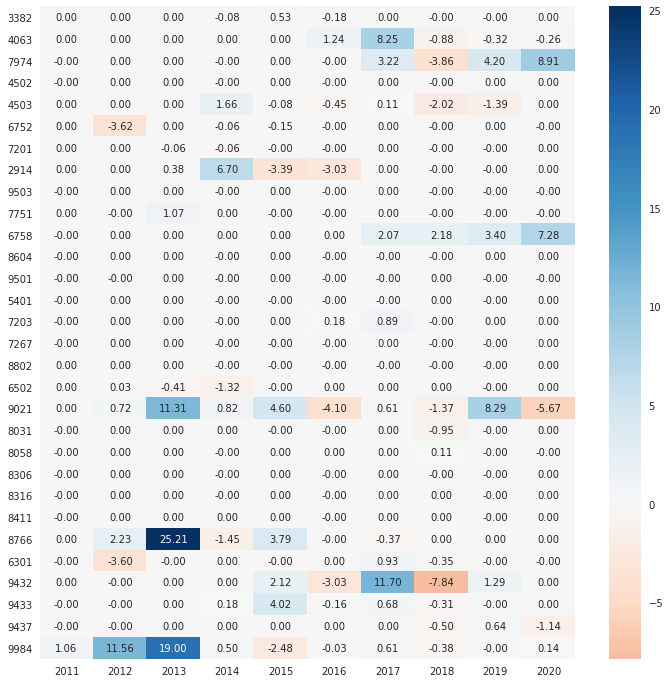
\includegraphics[width=0.8\hsize]{./figures/srmp_tpx30_w=60_hm.png}
\end{center}
\caption{\small 各銘柄の年次収益率(\%) シャープレシオ最大化モデル(TPX C30構成銘柄, 推定期間:60カ月)}
\label{fig:32}
\end{minipage}
\end{figure}

\end{document}